\documentclass{article}

\usepackage[utf8]{inputenc}
\usepackage[T1]{fontenc}
\usepackage[greek,english]{babel}
\usepackage{alphabeta}
\usepackage{amsmath}
\usepackage{amssymb}
\usepackage{graphicx}
\usepackage{subcaption}
\usepackage{epstopdf}
\usepackage[margin=1in, paperwidth=7.5in,paperheight=10.5in]{geometry}


\newcommand\course{ΤΗΛ513}
\newcommand\courseName{Δορυφορικές Ζεύξεις}
\newcommand\semester{Εαρινό 2020}
\newcommand\assignmentNumber{Lab 4 Δορυφορικών Επικοινωνιών}
\newcommand\studentName{Μαυρογιώργης Δημήτρης}                           
\newcommand\studentNumber{2016030016}

\title{\underline{\textbf{\assignmentNumber}}} 
\author{\textsc{\textbf{Όνομα:}}  \studentName\\
		\textsc{\textbf{ΑΜ:}}  \studentNumber\\
		\course \ - \courseName\\ 
		\textsc{Πολυτεχνείο Κρήτης}
}
\date{\today}
\begin{document}
	\maketitle
\section{Εισαγωγή}
Σκοπός της άσκησης είναι η εφαρμογή του αλγόριθμου Viterbi για την αποκωδικοποίηση ενός συνελικτικού κώδικα, ο οποίος θα χρησιμοποιηθεί για την
διόρθωση σφαλμάτων (forward error correction - FEC) κατά την μετάδοση κάποιων bit μέσα από ένα κανάλι BSC (binary symmetric channel). \\

\noindent
Πιο συγκεκριμένα, έστω ότι θέλουμε να μεταδόσουμε Ν  bits πληροφορίας $m_{1}, m_{2}, \dots m_{N}$ με $m_{i} \in \{0,1\}$, τα οποία αντιστοιχούν με κατάλληλη FEC
κωδικοποίηση, σε μία νέα ακολουθία από bits  $b_{1}, b_{2}, \dots b_{N}$ με $b_{i} \in \{0,1\}$. Συνεπώς, με την κωδικοποίηση εισάγουμε επιπλέον bits και για κάθε N bits πληροφορίας απαιτούνται 2Ν-1 bits, δηλαδή. ο ρυθμός της κωδικοποίησης είναι $ρ = \frac{N}{2N-1} \approx \frac{1}{2}$\\

\begin{figure}[h]
	\centering
	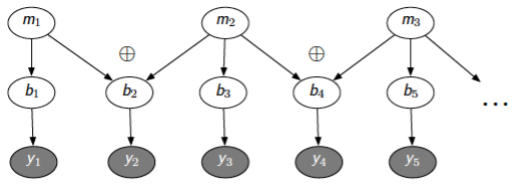
\includegraphics[width=0.5\linewidth]{./results/BSC_coding.png}
	\caption{Κωδικοποίηση με συνελικτικό κώδικα και μεταφορά μέσω καναλιού BSC}
\end{figure}
\noindent
Για την κωδικωποίηση των $m_{i}$ bits που θέλουμε να στείλουμε, θα χρησιμοποιήσουμε μια απλή μορφή συνελικτικού κώδικα με μήκος εξαναγκασμού L=2 και ρυθμό ρ=1/2, ο οποίος περιγράφεται ως εξής:
$$b_{2i-1} = m_{i} \ \ \ \ \ και \ \ \ \ \ b_{2i} = m_{i} \oplus m_{i+1} $$
όπου $\oplus$ είναι η πράξη xor και $i=1,2,\dots,N$\\

\noindent
Στην συνέχεια, τα κωδικοποιημένα bits $b_{i}$, με $i=1,2,\dots,2N-1$, εισέρχονται από ένα BSC κανάλι, το οποίο αλλάζει τo κάθε bit με πιθανότητα $ε \in (0,1/2)$, ενώ δεν το μεταβάλλει με πιθανότητα 1-ε. Οπότε, προκύπτει η ακολουθία εξόδου $y_{i}$, με $i=1,2,\dots,2N-1$. \\

\pagebreak
\noindent
Επιπλέον, γνωρίζουμε ότι η χωρητικότητα του παραπάνω καναλιού δίνεται από τη σχέση:
$$C_{BSC} = 1 - H(ε)$$
όπου H(ε) είναι η εντοπία μιας δυαδικής πηγής πληροφορίας και ισούται εξ'ορισμού με: 
$$H(ε) = -ε\log_{2}{(ε)} -(1-ε)\log_{2}{(1-ε)}$$

\begin{figure}[h]
	\centering
	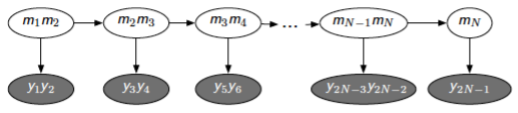
\includegraphics[width=0.6\linewidth]{./results/BSC_coding1.png}
	\caption{Απλοποίηση της παραπάνω κωδικοποίησης και μεταφοράς σε ένα ισοδύναμο HMM }
\end{figure}

\noindent
Από τη θεωρία πιθανοτικών γραφικών μοντέλων αποδεικνύεται ότι το figure 1 μπορεί να απλοποιηθεί στο hidden Markov model (figure 2). Επιπλέον, προκύπτει ότι παρατηρώντας τα σύμβολα $(y_{2i-1},y_{2i})$ μπορούμε να καταλάβουμε ποιο ζεύγος $(m_{i},m_{i+1})$ στάλθηκε.\\

\noindent
Κατα την αποκωδικοποίηση του συνελικτικού κώδικα, χρησιμοιποιούμε τον κανόνα maximum likelihood-ML, προσπαθώντας να μεγιστοποιήσουμε την εξής πιθανότητα:
$$Pr(y_{1},\dots,y_{2N-1}|m_{1},\dots m_{N}) \propto Pr(y_{2N-1}|m_{N})\prod_{i=1}^{N-1} Pr(y_{2i-1},y_{2i}|m_{i},m_{i+1})$$
Επιπλέον, αν χρησιμοποιήσουμε και την ιδιότητα των λογαρίθμων, προσπαθούμε να μεγιστοποιήσουμε το άθροισμα των λογαρίθμων. \\
Συνεπώς, αν κατασκεβάσουμε το trellis με βάρη που προκύπτουν από τον παραπάνω κανόνα ML, μπορούμε  να χρησιμοποιήσουμε τον αλγόριθμο Viterbi για την αποκωδικοποίηση του παραπάνω συνελικτικού κώδικα.

\pagebreak
\section{Eρώτημα 1}
Για τιμή ε=1/5 και Ν=128 bits δημιουργούμε την ακολουθία $y_{1}, y_{2}, \dots y_{2N-1}$, όπως περιγράφτηκε παραπάνω, και καταλλήγουμε στο συμπέρασμα ότι εκτιμήθηκαν λανθασμένα περίπου 19 bits. Aν επαναλάβουμε για $10^4$ φορές προκύπτει ότι το BER για ε=1/5 είναι περίπου 0.1896.\\

\section{Eρώτημα 2}
Aν επαναλάβουμε τη διαδικασία για ε=1/6, ε=1/8, ε=1/10 και ε=1/20, προκύπτει ότι τα bits που εκτιμήθηκαν λάθος έιναι 18, 12, 9 και 2 αντίστοιχα. Επαναλαμβάνοντας για $10^4$ φορές και τις τις παραπάνω τιμές πιθανότητας ε, εκτιμήθηκε το BER περίπου ίσο με 0.1443, 0.0907, 0.0625 και 0.0188 αντίστοιχα. Επιπλέον, προκύπτει το παρακάτω διάγραμμα BER συναρτήση του ε σε λογαριθμική κλίμακα. 
\begin{figure}[h]
	\centering
	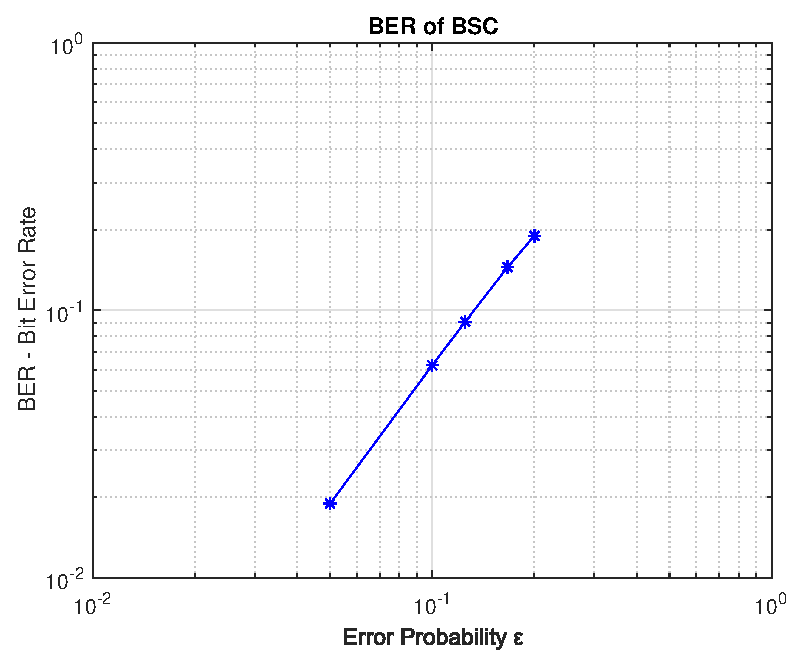
\includegraphics[width=0.6\linewidth]{./results/lab4eps.eps}
\end{figure}

\section{Eρώτημα 3}
Aπό το παραπάνω διάγραμμα παρατηρούμε ότι όσο μειώνεται η πιθανότητα ε, μειώνεται και και το BER στο κανάλι BSC. Ειδικότερα, γίνεται αντιληπτό ότι ο λογάριθμος του BER είναι ανάλογος του λογαρίθμου της πιθανότητας σφάλματος ε.\\
Τέλος, παρατηρούμε ότι με τη μείωση του ε επηρρεάζει την εντροπία της πηγής πληροφορίας H(ε). Πιο συγκεκριμένα η εντροπία, που αποτελεί ένα "μέτρο αβεβαιότητας" για το τηλεπικοινωνιακό σύστημα, μειώνεται, με αποτέλεσμα η συνολική χωρητικότητα του καναλιού να αυξάνεται.


\end{document}
